\chapter{THE HYDROGENIC ISO-SEQUENCE}
% !TEX root = hazy3.tex

Tests in the low-density, or nebular, limit show that the model atom predicts
level populations and emissivities that are in much better than 1\% agreement
with Seaton (1959), and with the Storey and Hummer (1995) results.  The
atom goes to LTE in the high radiation or matter density limits.

\section{Recombination rates and cooling}

\subsection{Rational approximations}%[gjf1]

It is not numerically expedient to compute these rate coefficients on-the-fly
in large scale ionization/thermal structure calculations.  The rate
coefficients were fitted with a high-order rational approximation.  The
recombination rate coefficient is expressed~as
\begin{equation}
\alpha \left( {n,T} \right) = {10^{F(n,T)}}\;{T^{ - 1}}
\end{equation}
with
\begin{equation}
F(n,T) = \frac{{{a_n} + {c_n}x + {e_n}{x^2} + {g_n}{x^3} + {i_n}{x^4}}}{{1
+ {b_n}x + {d_n}{x^2} + {f_n}{x^3} + {h_n}{x^4}}}
\end{equation}
and $x \equiv \log$(T).  These approximations reproduce the numerical results with
a mean error well below 0.1 percent.  For levels below $n=20$ the largest
error is also under 0.1 percent, although errors as large as 1.4 percent
occur for the highest sum at temperatures below 100~K.

Recombination cooling coefficients were fitted to equations of the form
\begin{equation}
kT\beta \left( {n,T} \right) = {10^{F(n,T)}}
\end{equation}
where $F(T,n)$ is given above, and the fitting coefficients are given in the
code.  The errors in fitting these coefficients are larger, typically 0.5
percent, but sometimes as large as several percent.

\section{Effective transition probabilities}

\subsection{Einstein As}

Two routines are used to compute hydrogenic transition probabilities, in
the limit of a completely $l$-mixed atom.  There routines were coded by Jason
Ferguson, using algorithms given by \citet{Johnson1972}.

Note that the code considers the $2s$ and $2p$ as two separate levels.  These
routines return transition probabilities for a well $l$-mixed atom, and cannot
be applied directly to the separate $2s$ and $2p$ levels.

\section{Collisional contributions to hydrogen lines}

Figure \ref{fig:HLinesFerlandOsterbrock},
taken from Ferland \& Osterbrock (1985), shows the effects of
collisional excitation on hydrogen lines.  This process can be significant
relative to recombination when the gas temperature is high (perhaps due
to low metallicity) or in partially neutral gas that is exposed to x-rays.
The lines marked ``external'' are reddening curves due to external dust,
and ``internal'' tracks the effects of internal dust.  The band of solutions
that go across the top of the figure shows the expected hydrogen line
spectrum, as set by the collision strengths of the Lyman lines.

\begin{figure}
\centering
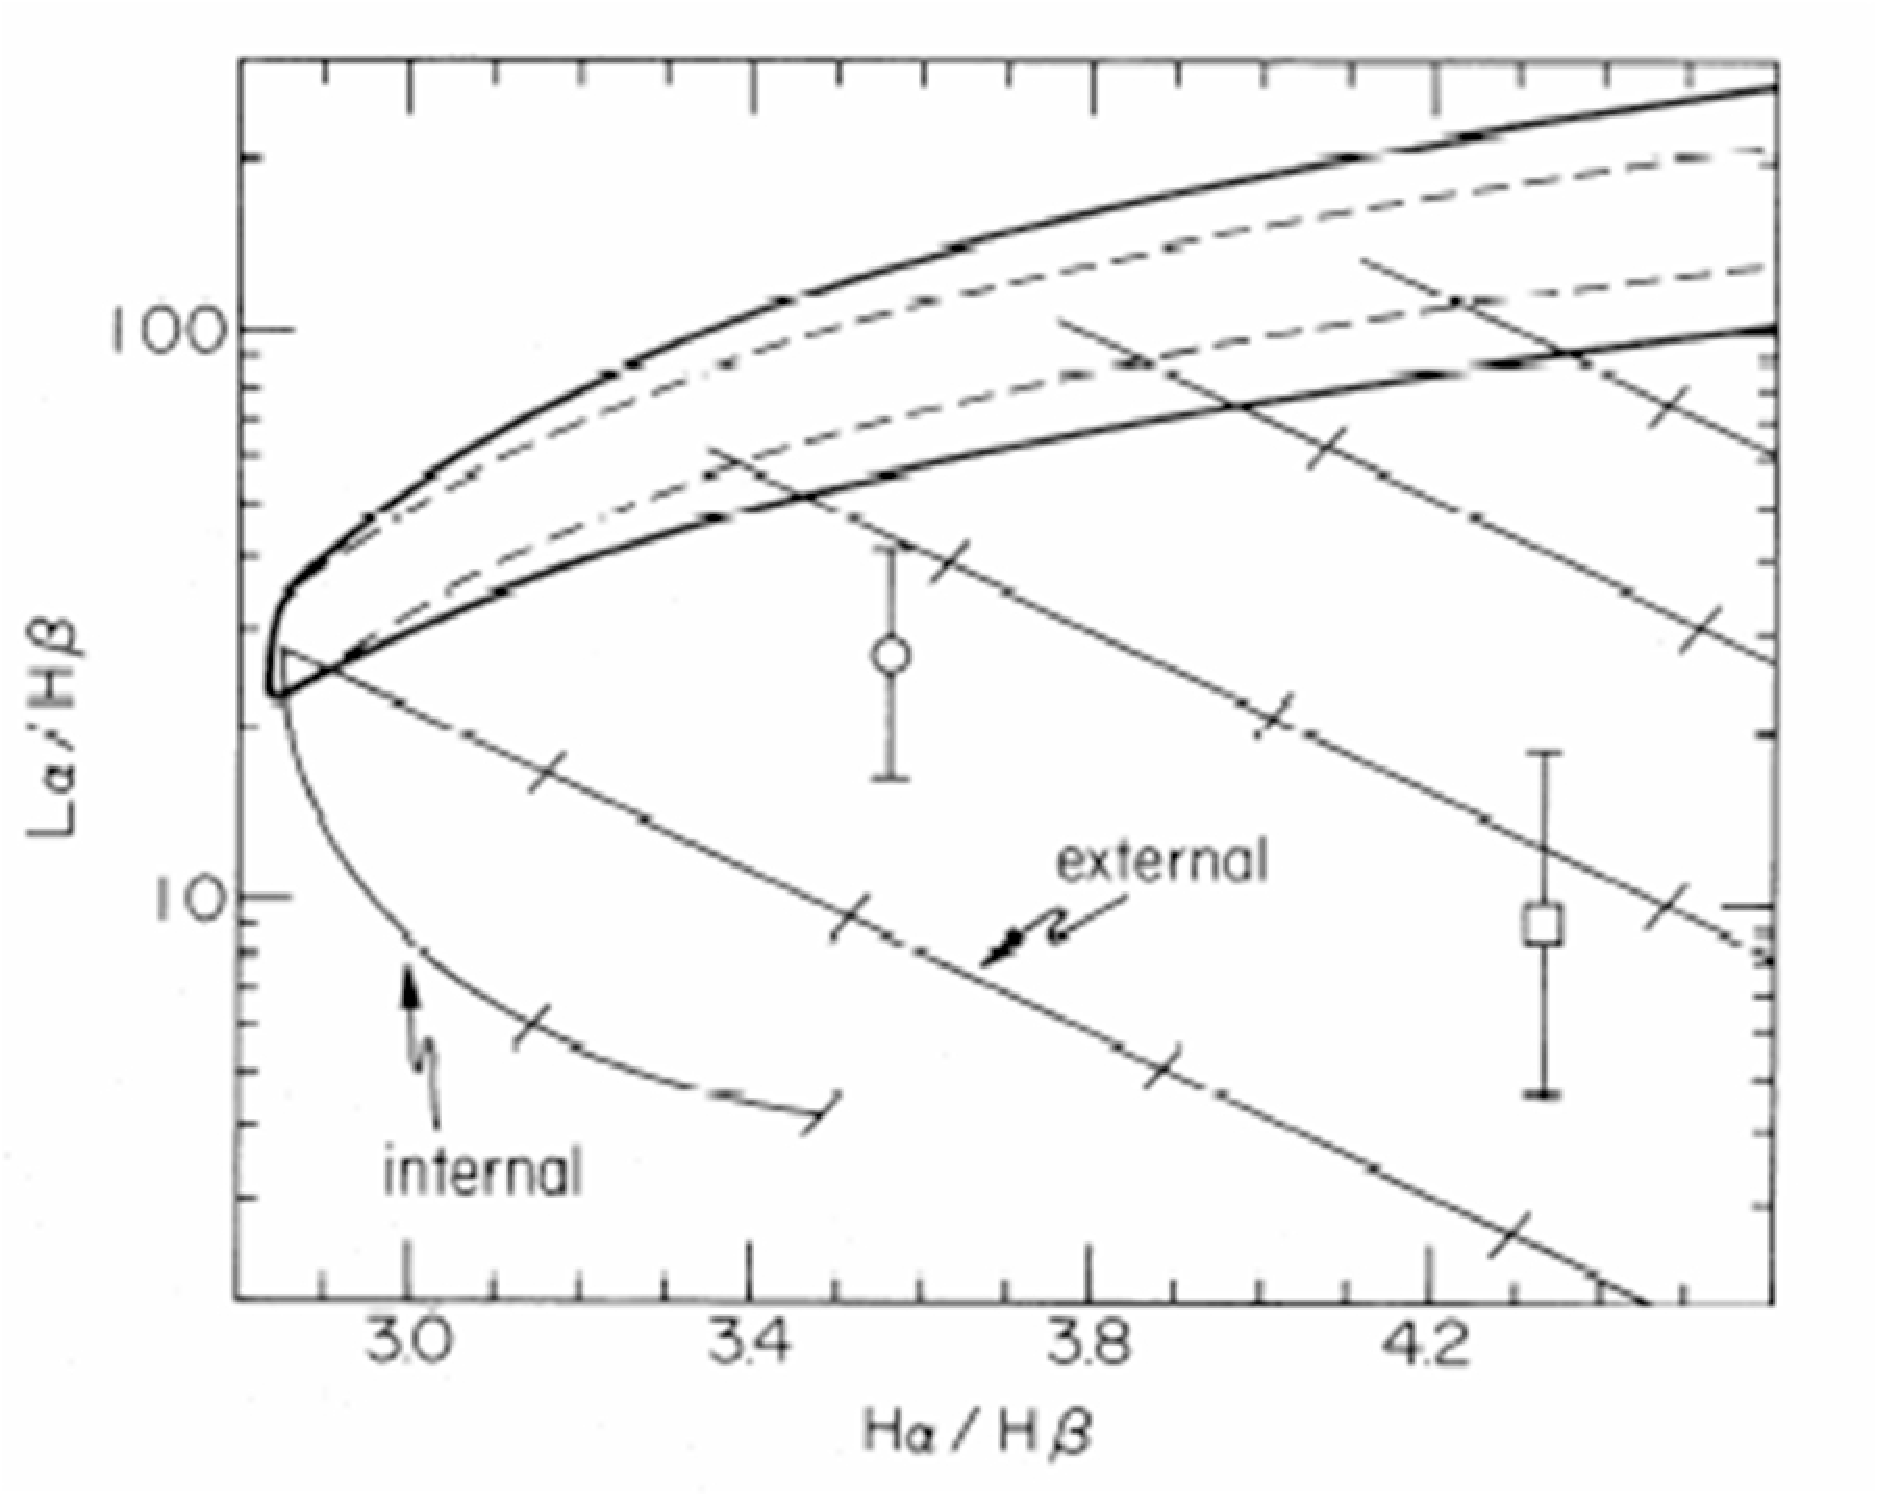
\includegraphics[scale=0.4]{HLinesFerlandOsterbrock}
\label{fig:HLinesFerlandOsterbrock}
\caption[Hydrogen line ratios]
{This figure, taken from Ferland \& Osterbrock 1985, shows the
effects of collisional excitation upon two ratios of hydrogen lines.  The
largest effects are to enhance \la\ and \ha\ by large amounts. }
\end{figure}

\section{Continuous thermal emission}

Diffuse emission (free-free and free-bound) by all atoms is computed using
the stored photoabsorption cross sections and detailed balance (i.e., the
Milne relation; see \citealp{Mihalas1978}).

Free-bound continua of all levels of hydrogen and helium are treated as
follows.  The Milne relation for the emissivity $4\pi j$ (erg~cm$^3$
Hz$^{-1}$~s$^{-1}$) can
be expressed as (Brown and Mathews 1970)
\begin{equation}
r\pi j_\nu = h\nu \left(\frac{2\pi m_ck}{h^2}\right)^{3/2} \frac{8\pi}{c^2}
\frac{g_n}{g_eg_{ion}} T^{-3/2}\nu^2 \alpha_\nu (n) \exp
\left(-h(\nu-\nu_o)/kT\right)
\end{equation}
where the statistical weight of level $n$ is $g_n = 2n^2$ for $H^0$ and
He$^+$, and
$g_n = n^2$ for helium singlets.

The code actually works with units similar to photons
Ryd$^{-1}$~s$^{-1}$~cm$^{-2}$.  The
photon emissivity (photons cm$^3$ s$^{-1}$ Ryd$^{-1}$) is then
\begin{equation}
\label{eqn:HPhotonEmissivity}
\begin{array}{ccc}
 {\varphi _\nu }\left( {T,n} \right)&  =& {\left( {\frac{{2\pi
\,{m_e}k}}{{{h^2}}}} \right)^{ - 3/2}}\;\frac{{8\pi
}}{{{c^2}}}\;\frac{{{g_n}}}{{{g_e}{g_{ion}}}}\;{T^{ - 3/2}}\;{\nu ^2}{\alpha
_\nu }\left( n \right)\exp \left( { - h\left( {\nu  - {\nu _o}} \right)/kT}
\right) \\
&=& 4.12373 \times {10^{11}}\frac{{{g_n}}}{{{g_e}{g_{ion}}}}\;{T^{ -
3/2}}\;{\nu _{Ryd}}^2{\alpha _\nu }\left( n \right)\,\exp \left( { - h\left(
{\nu  - {\nu _o}} \right)/kT} \right) \\
 \end{array}
\end{equation}
where the $g$'s are the statistical weights of the constituents, $\nu_{Ryd}$ is the
photon energy in Rydbergs, $h\nu_o\sim z^2/n^2$ is the ionization potential in Rydbergs,
$\alpha_\nu(n)$ is the photoionization cross section, and the other symbols have their
usual meanings.
Equation \ref{eqn:HPhotonEmissivity} is evaluated directly using the stored
photoionization cross sections.  A similar approach is used for all
absorption opacities.  Detailed balancing between absorption and emission
mechanisms is necessary if LTE is to be achieved.

A test case with an ionized hydrogen plasma at a temperature
of $10^4 \K$ and
a density of $10^7~\pcc$
(to suppress two photon emission) was computed, and
is shown in Figure~\ref{fig:HemisCompareFerland80}.

\begin{figure}
\centering
\label{fig:HemisCompareFerland80}
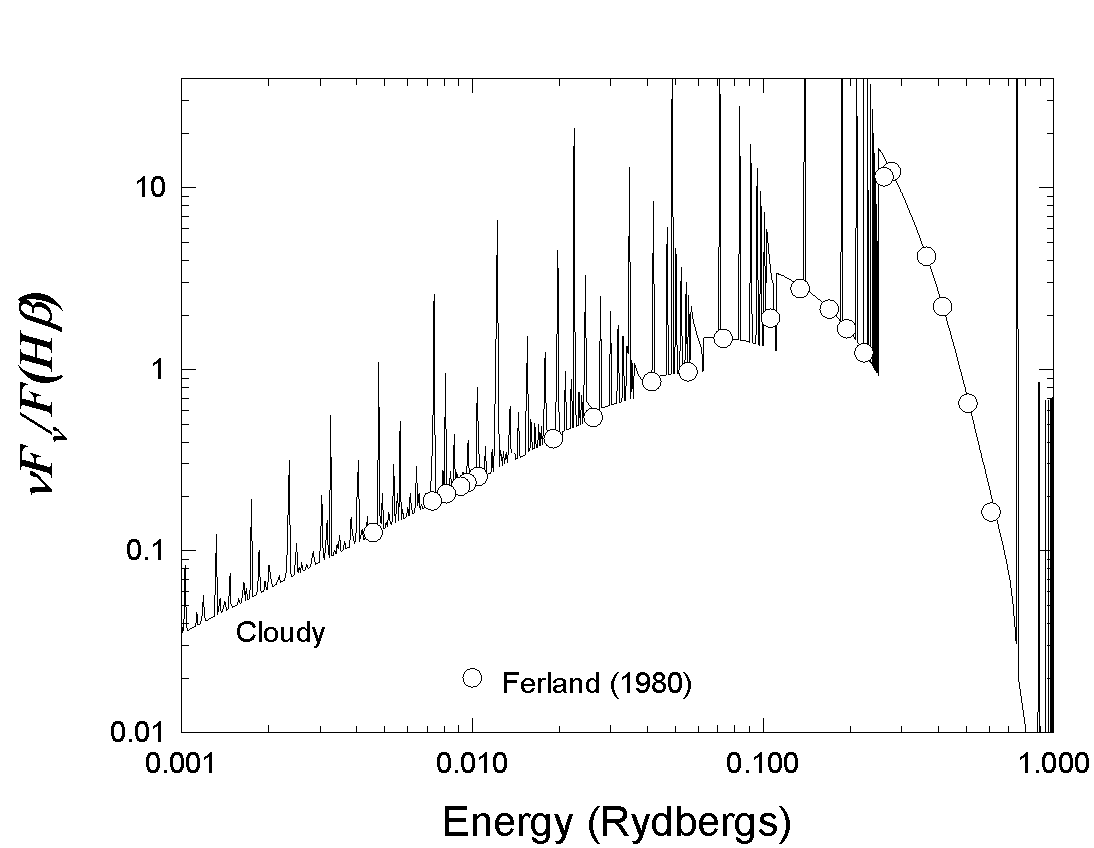
\includegraphics[scale=0.8]{HemisCompareFerland80}
\caption[H emission comparision]{The emission from a slab of gas is compared with the
predictions of Ferland (1980).}%  hemis computed Page: 212
\end{figure}
%97 jan 3, using 90.02l

The input stream used to derive the figure is included in the test suite.
As can be seen from this figure, the predicted diffuse continuum is generally
within a percent of the exact value (given in Ferland 1980).

Figure \ref{fig:HConEmissBBLimit} shows another series of test cases in which a very high density
gas with cosmic abundances is irradiated with a 50,000 K blackbody radiation
field in strict thermodynamic equilibrium.  As can be seen from the figure,
the predicted continuum goes to the blackbody limit.

%Figure 4
\begin{figure}
\label{fig:HConEmissBBLimit}
\centering
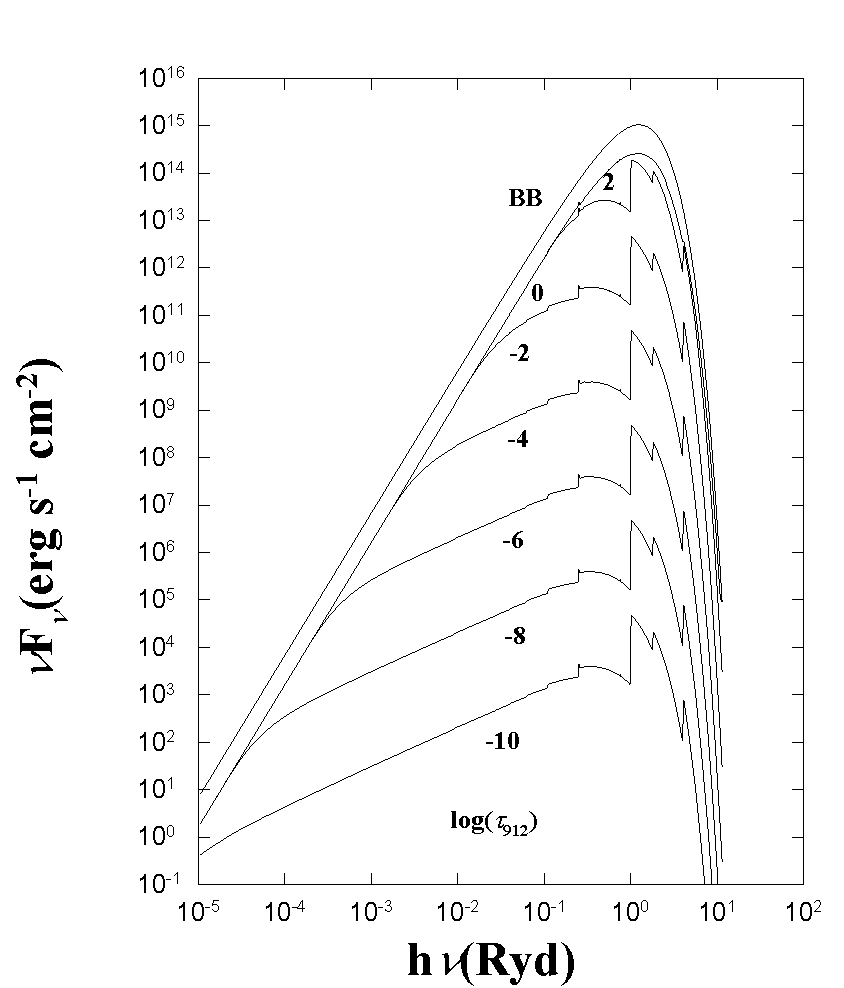
\includegraphics{HConEmissBBLimit}
\caption[H emission in black body limit]
{The emission from a dense slab of gas with cosmic abundances is
shown as a function of the optical depth at the Lyman limit.  The log of
this optical depth is indicated on the figure.  The top curve is for emission
given by Planck's law.  The continuous emission goes to the blackbody limit
in the case of large continuum optical depths.}
\end{figure}

